\documentclass[sigconf]{acmart}

%%
%% \BibTeX command to typeset BibTeX logo in the docs
\AtBeginDocument{%
  \providecommand\BibTeX{{%
    \normalfont B\kern-0.5em{\scshape i\kern-0.25em b}\kern-0.8em\TeX}}}

\usepackage[margin=0.5in]{geometry}
\usepackage[utf8]{inputenc}
\usepackage{graphicx}

\begin{document}

%%
%% The "title" command has an optional parameter,
%% allowing the author to define a "short title" to be used in page headers.
\title{Big data final project}

%%
%% The "author" command and its associated commands are used to define
%% the authors and their affiliations.
%% Of note is the shared affiliation of the first two authors, and the
%% "authornote" and "authornotemark" commands
%% used to denote shared contribution to the research.
\author{Hechun Wang}
\email{hw1964@nyu.edu}
\affiliation{%
  \institution{New York University}
  \city{New York}
  \state{NY}
  \postcode{11201}
}

\author{Kaixuan Zhou}
\email{kz1005@nyu.edu}
\affiliation{%
  \institution{New York University}
  \city{New York}
  \state{NY}
  \postcode{11201}
}

\author{Min Yang}
\email{yangmin05235@outlook.com}
\affiliation{%
  \institution{New York University}
  \city{New York}
  \state{NY}
  \postcode{11201}
}


%%
%% The abstract is a short summary of the work to be presented in the
%% article.
\begin{abstract}
This report details the process of 3 tasks to profile a large collection of open datasets from NYC Opendata and derive metadata that can be used for data discovery, querying and identification of data quality problems. The 3 tasks are to perform generic profiling of 1900 tables, perform semantic profiling on 270 tables to create a prediction algorithm for labelling and perform data analysis on 311 complains.
In order to perform the tasks, the following data analysis methods are performed:
\begin{itemize}
\item {\verb|Data cleaning|}: Processing table names, column names and column content before processing
\item {\verb|Data processing|}: Processing large volume data using map-reduce and spark
\item {\verb|Data explanation|}: Aggregate the processed data and explain the result
\end{itemize}
The findings and results of the tasks are presented in the content below. 
\end{abstract}



%%
%% This command processes the author and affiliation and title
%% information and builds the first part of the formatted document.
\maketitle

\section{Introduction}
The motivation for this project is to implement big data processing methodologies on NYC Opendata dataset to profile a large volume of data with great efficiency and accuracy. The following problems are faced in the process:
\begin{itemize}
    \item Bad data in values such as invalid characters or bad representation of data(e.g. N/A, Null in a column of numbers)
    \item Processing a large volume dataset in a relative short amount of time
    \item perform labelling prediction on columns according to the values of the cells in the column
\end{itemize}

The problems stated above are important for data processing because they each generate devastating effects to the whole process. Bad data will render errors in the processing phase and generate bad results. Using local processing instead of cluster processing will never generate the required results in time. And of course the best results are required from any prediction algorithm to align with the actual labels of each column.

The underlying concept to solve each problem are:
\begin{itemize}
    \item Replace and clean invalid characters in each column and unify cells with the same type. 
    \item Use map-reduce and spark to process the data in parallel and minimum time
    \item Use dictionary, regex and other semantic labelling method to generate a reliable prediction model
\end{itemize}

By utilizing the concepts above, we can generate reliable results in minimum time with maximum efficiency. The results given are much better comparing to running them on one or several personal workstations. The results are also human readable and better prone to evaluation and explanation.


%%%%%%%%%%%%%%%%%%%%%%%%%%%%%%%%%%%%%%%%%%%%% below this line is Task1%%%%%%%%%%%%%%%%%%%%%%%%%%%%%%%%%%%%%%%%%%%%%
\section{Task1: Generic Profiling}
In this task,  we are to profile the data sets and derive metadata that can be used for data discovery, querying, and identification of data quality problems. For each column, it should be labelled with the following attributes:
\begin{itemize}
    \item Number of non-empty cells
    \item Number of empty cells
    \item Number of distinct values
    \item Top-5 most frequent value(s)
    \item Data types (a column may contain values belonging to multiple types)
    \begin{itemize}
        \item INTEGER (LONG)
        \item REAL
        \item DATE/TIME
        \item TEXT
    \end{itemize}
\end{itemize}

We successfully gathered the required metadata for 1891 datasets (out of 1900). The remaining datasets either takes too long for us to compute, or has some data error such as 'int too large to convert to float'. The unprocessed files are also recorded for future optimization in the team's GitHub directory.

The output of the labeling process is one JSON files, which contains all the metadata for the 1891 datasets. The output file can be found in our GitHub repository under the result folder.
\subsection{Challenges and Optimization}
In this subsection we are going to discuss some challenges we face along the way, and some solutions and optimizations we have applied to tackle the respective challenges.
\subsubsection{Spark and Spark-SQL}
As we finished the initial version of the program, we found out that the program is taking longer than expected. After team member's review, it appears that we are doing a lot of duplicated work. We used a different spark-sql query for a different task without extracting the data needed in common and reduce the cost of computing.
\begin{itemize}
    \item The total number of cells, the number of empty cells, and the number of not empty cells were counted for every column in the same dataset.
    \item When we were to find the number of distinct values and top-5 most frequent values, we have two queries for them, and those two queries are doing some duplicated work.
\end{itemize}
As a solution to optimize:
\begin{itemize}
    \item We only count the number of rows for one dataset once, and we count the number of non-empty rows for each column. Then, with a simple subtraction, we get the number of empty rows.
    \item We perform a groupby operation. While we are looking for the number of distinct values, we can also maintain the number of occurrence for each distinct value. We can then perform a sortby opeartion to find the top-5 most frequent values.
    \item We change the code from pyspark-sql to pyspark so that it's easy to read and maintain since pyspark-sql query is genrally longer.
\end{itemize}
\subsubsection{Ways to initiate a spark job}
As our first approach, A bash script was used to submit one pyspark job per dataset. As we collect the data, we realize that for each submitted work, it takes around 60 - 120 seconds to set up the spark context, and it's even longer when Dumbo is under a high usage. 
We then used a nested for loop inside the python script to iterate through all the dataset and all the columns in each dataset.
\subsubsection{Long time to profile the data}
We seperate the task into three portions, and each team member runs one third of the entire task. We maintain a task bank which contains all the task each team member needs to run for TASK 1. We also realized that after a certain time without I/O, dumbo will terminate the session automatically. To handle that, an output indicating which stage of the task is on right now will be printed out after a certain amount of time.erkler
\subsubsection{Fault tolerance}
While we are running the code, we sometimes need to update the script to encounter some unforeseen errors. In order to not rerun the already profiled dataset, we will remove the task from the task bank.
\subsubsection{Miss-classification of "DATE/TIME"}
We are using a package "dateutil.parser" to parse the column value if the default type given by spark is string. However, we decided to detect if it's an INTEGER first, then REAL, then DATE/TIME, and finally TEXT. That leads to some situations when:
\begin{itemize}
    \item If the given string is "20191209", our type checker would determine this as an INTEGER, rather than a date.
    \item The parser will also classify string looks like "140ST" as "0140-12-05 00:00:00". However, the team didn't notice this issue until 80\% of the data sets are already profiled. This can be solved by manually looking at the co-occured datatype. If DATE/TIME co-occurs with TEXT and INT, that could mean the input data is not problematic.
\end{itemize}
We treat these as our features. However, because of the ignorance of the above situations, the json output will have the largest DATE and the lowest DATE value being the parsed "DATETIME" object rather than the original string stored in the database. This output format was fixed soon after the team realized the defect, and the codebase is already updated. However, the output gathered previously was not updated due to time limit (the team didn't rerun the code for the profiled datasets).
\subsection{Data Quality Issues}
In this subsection, we will discuss some data quality issues that the project team faced while profiling the data.
\subsubsection{Too many empty and wrong values} As shown in Figure 1: Among the 38375 columns, 66\% of those have NULL being the top-5 most frequent values, and 80\% of those have NULL as most frequent value. There are also a lot of "wrong" values. For example, a "Y...." in a column containing some color information, and a 2 digit zip code, etc.
\begin{figure}[htp]
    \centering
    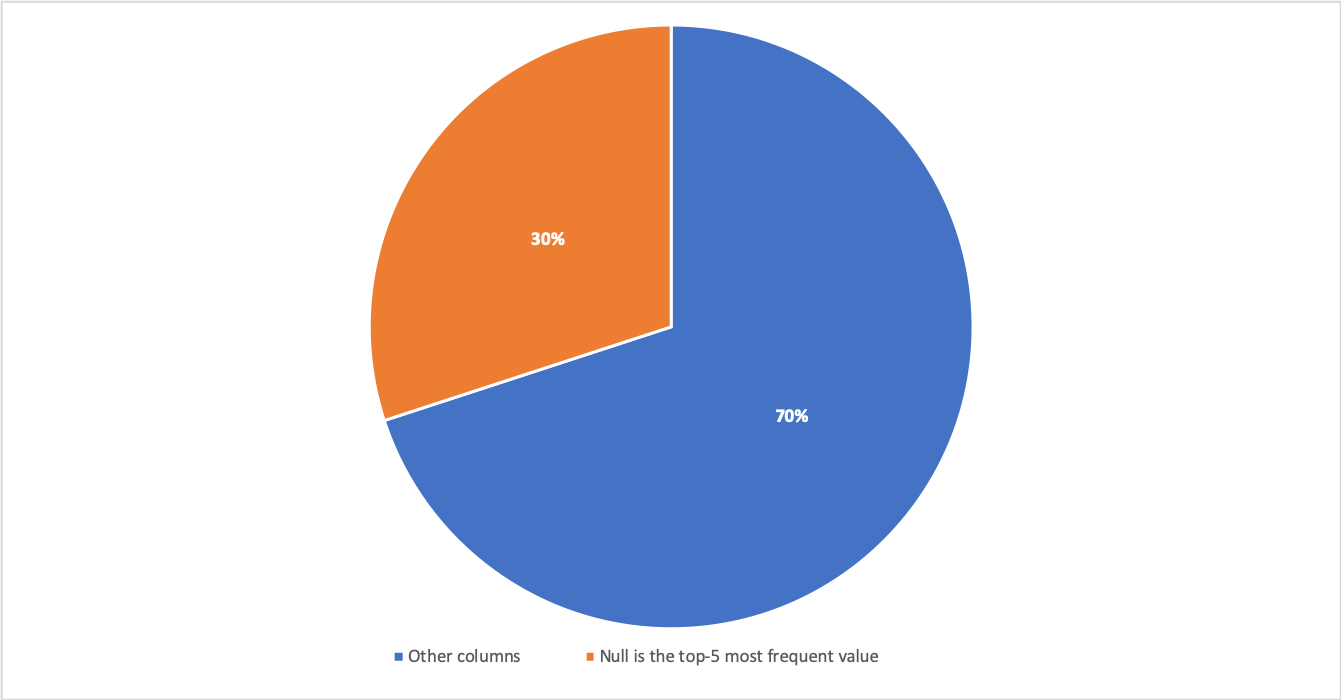
\includegraphics[width=8cm]{null_col.png}
    \caption{Column Distribution}
    \label{fig:galaxy}
\end{figure}
\subsubsection{heterogeneous Columns} There are 28007 columns has only one data type. The number of columns that has 2, 3, 4 data types are: 6644, 1556, 2168, respectively. Shown in Figure 2.
\begin{figure}[htp]
    \centering
    \includegraphics[width=7cm]{col_types.png}
    \caption{Column Data Types Distribution}
    \label{fig:galaxy}
\end{figure}
\subsubsection{Miss-classification of "DATE/TIME"} Follow up on heterogeneous columns: Referring to the previous section, the reason why our type checker miss clasified the data is because the data is not entered in a unified way, and actually we cannot tell if "18880101" is a datetime or some random number; and "2019/04" is a datetime or not unless we look at the column name, or the other values in the column in general.
\subsubsection{Redundant Column Name} The dataset also contains some extraordinarily long column names. The longest column name contains 225 characters, it is:
\begin{itemize}
    \item 'Part Time Licensed PE Teachers - Itinerant PE Teachers - As of 10/31/2015 (APE teachers not included) - Elementary, Early Childhood, and K-8 teachers providing physical education under a common branch license are not included'
\end{itemize}

\subsection{Data Exploration and Visualization}
\subsubsection{Time needed to profile the datasets}
\begin{figure}[htp]
    \centering
    \includegraphics[width=8.5cm]{time_elapsed_min.png}
    \caption{Time Elapsed Less than 1 hour}
    \label{fig:galaxy}
\end{figure}
\begin{figure}[htp]
    \centering
    \includegraphics[width=8.5cm]{time_elapsed_hour.png}
    \caption{Time Elapsed more than 1 hour}
    \label{fig:galaxy}
\end{figure}
Figure 3 only shows the time needed for those files that took less than 60 minutes to process (95\% of the datasets takes less than 1 hour to process.) From Figure 3, we can clearly see that the majority of the datasets takes less than 20 minutes to process. Figure 4 shows the time elapsed for files that take more than an hour to process. The dataset that takes the longest to process is "mmvm-mvi3". It takes around 5.8 hour to process.
\subsubsection{Extra Credit: Key column candidate} The team took a naive approach to identify the key column candidate: If a column has number of distinct values equal to the total number of rows of the dataset, then this column is one of the key column candidate. This approach doesn't consider the situation when a composite key is allowed. That is, this approach can only handle the situation when there is one primary key. With this naive approach, the team found out that 806 datasets have a primary key potentially, which means roughly 40\% of the datasets have a index column.
\subsubsection{Detailed data report} In this subsection, we are going to discuss the general data layout for the datasets. For the four different data types: INT, REAL, DATE/TIME, and TEXT, the global max and min are:
\begin{itemize}
    \item INT: \textasciitilde$10^{100}, -14248677237$
    \item REAL: inf, -469079690.9
    \item DATE/TIME: 0001-01-01, 9999-12-31
    \item len(TEXT): 32759, 1
\end{itemize}
\begin{figure}[htp]
    \centering
    \includegraphics[width=8.5cm]{int_mean.png}
    \caption{Integer (long) Mean Distribution}
    \label{fig:galaxy}
\end{figure}
\begin{figure}[htp]
    \centering
    \includegraphics[width=8.5cm]{dates_distribution.png}
    \caption{Dates Distribution}
    \label{fig:galaxy}
\end{figure}
\begin{figure}[htp]
    \centering
    \includegraphics[width=8.5cm]{avg_text_length.png}
    \caption{Average Text Length}
    \label{fig:galaxy}
\end{figure}
For simplicity, we only show the significant data rather than the entire dataset. For Figure 6, we only showed the dates that occur later than year 2008. For Figure 5 and 7, we only show the means that is from the range (-100, 2300), and for better visualization, we only limit the y range as well.

From the graphs, we can see that there are two peaks in the integer mean distribution. One is near 0, and the other one is near 2000. We can also tell that most of the dates are around 2014. And the majority of the average length are less than 25. There are 4311 columns with type TEXT have an average length of 1.
\subsubsection{Frequent itemset analysis}
\begin{table}
  \caption{Frequent Itemset}
  \label{tab:freq}
  \begin{tabular}{{l l}}
    \toprule
    Data Types& Support\\
    \midrule
    A: Text& 19934\\
    B: Integer (long)& 21711\\
    C: Real& 1722\\
    D: Date/Time& 4008\\
    \midrule
    A \& B& 6358\\
    A \& C& 1713\\
    A \& D& 2638\\
    B \& C& 914\\
    B \& D& 1365\\
    C \& D& 442\\
    \midrule
    A \& B \& C& 909\\
    A \& C \& D& 433\\
    A \& B \& D& 1268\\
    B \& C \& D& 358\\
    \midrule
    A \& B \& C \& D& 353\\
  \bottomrule
\end{tabular}
\end{table}
In the section, we found the 2,3,4-frequent itemsets from the generated metadata. Noticed that it might have some errors according to the previous two sections. Refer to Table 1, given a min-support of 1000, and a min-confidence of 60\%, the 2,3,4-frequent itemsets are:

\begin{itemize}
    \item Text and Date/Time.
        \subitem  Support: 2638, Confidence: 65.8\%
    \item Text, Integer (long) and Date/Time.
        \subitem Support: 1268, Confidence: 92.9\% 
    \item Text and Real.
        \subitem  Support: 1713, Confidence: 99.5\%
\end{itemize}


%%%%%%%%%%%%%%%%%%%%%%%%%%%%%%%%%%%%%%%%%%%%% below this line is Task2%%%%%%%%%%%%%%%%%%%%%%%%%%%%%%%%%%%%%%%%%%%%%
\section{Task2: Semantic Profiling}
In this task, we are to extract detailed information about the semantics for 270 given columns. For each column, it should be labelled with one or more of the following labels:
\begin{itemize}
\item Person name
\item Business name
\item Phone Number
\item Address
\item Street name
\item City
\item Neighborhood
\item LAT/LON coordinates
\item Zip code
\item Borough
\item School name
\item Color
\item Car make
\item City agency
\item Areas of study
\item Subjects in school
\item School Levels
\item College/University names
\item Websites
\item Building Classification
\item Vehicle Type
\item Type of location
\item Parks/Playgrounds
\item Other
\end{itemize}
After labelling, it is required for each semantic type identified, all the values encountered for that type are to be enumerated and presented in an aggregated collection. The output for this section can be found in our GitHub repository under the result folder.
\subsection{Preparations}
Before starting on the prediction model, the first step that must be taken is to label all the columns given by hand. The process to do this can be split into 3 steps:
\begin{itemize}
\item assigning each column with 1 label(most cases)
\item go through the column to find cells with different labels than the one labeled
\item cross identification by exchanging columns between different group members
\end{itemize}
\subsection{Strategies}
There are 3 strategies used in performing this section's task:
\begin{itemize}
\item Regex identification
\item column name dictionary identification
\item mixed identification
\end{itemize}
And each can be detailed in the following fashion:
\subsubsection{Regex identification}
This identification strategy is mainly used for detecting phone numbers, zip codes and Lat/Lon coordinates. Which are columns that contain values with strict formatting and can be identified using regular expression matching very easily. This identification strategy is performed using the following steps:
\begin{itemize}
\item Percolate the column and get the value of each cell
\item Use the value gotten from each cell and match the value to a specific regular expression type as phone number, zip codes and Lat/Lon coordinates and see if it gets a match  
\item If there is a match, we can assign the matching label to the column
\end{itemize}
\subsubsection{column name dictionary identification}
This identification strategy is mainly used for detecting columns with values that are not strictly formatted nor is small enough to use dictionary method on each cell's value. During the labelling stage, we discovered that most of the columns given contain a certain keyword within it's column name that could directly point to the main label of the column. For example table column \verb|2bnn-yakx_Vehicle_Color| contains the keyword color which can be used to directly label this column. This works for most columns given and can be done in the following steps:
\begin{itemize}
\item Design the dictionary of keywords that match to labels. For example "boro" is a match for the label "Borough"
\item Go through the columns assigned to us and clean the column name, turning every letter into lower case and removing any invalid characters apart from [a-z] and [0-9]
\item percolate the dictionary of keywords and check if each keyword are contained within the dictionary, if it is contained within the dictionary, assign the label to the column
\end{itemize}
\subsubsection{mixed identification}
By merging the two identification strategies together, we are able to perform an identification strategy that generates better result, the mixed identification process is relatively simple:
\begin{itemize}
\item Perform the column name dictionary identification on a column, and put any detected label into a predicted list
\item Go through the content of the column, and use regex identification on each of the cells and generate, if any labels that matches the regular expression.
\item For those columns that have no labels from the identifications combined, we assign a "Other" label to the column
\end{itemize}
\subsection{Benefits and limitations}
The benefits and limitations to the 3 different strategies are very clearly distinguished. For the Regex matching identification method, the benefits are that it could generate an almost 100\% accuracy for any cells containing formatted values. 
For the column name dictionary identification strategy, it would generate a very satisfying result for the columns that contain values with type string and unable to match regex or dictionary due to the large pool of distinct data they contain.
The limitations for each of the two strategies are that they can't perform task that the other could, making them two separate strategies that have to be combined together to get the whole picture. Another limitation of the two is that they can't generate multiple labels for a column individually.
To fix the limitations mentioned above, we merged them together into a mixed strategy that overcomes the limitations and can perform high accuracy detection of labels and able to generate multiple labels for one column to deliver the most satisfying result.
\subsection{Evaluation}
For each strategy, the precision and recall are:

\begin{figure}[htp]
    \centering
    \includegraphics[width=8cm]{ST2.png}
    \caption{result from Regex identification}
    \label{fig:galaxy}
\end{figure}
\begin{figure}[htp]
    \centering
    \includegraphics[width=8cm]{ST1-1.png}
    \caption{result from dictionary identification}
    \label{fig:galaxy}
\end{figure}
\begin{figure}[htp]
    \centering
    \includegraphics[width=8cm]{ST1-2.png}
    \caption{result from dictionary identification cont}
    \label{fig:galaxy}
\end{figure}
\begin{figure}[htp]
    \centering
    \includegraphics[width=8cm]{ST2-1.png}
    \caption{result from mixed identification}
    \label{fig:galaxy}
\end{figure}
\begin{figure}[htp]
    \centering
    \includegraphics[width=10cm]{ST2-2.png}
    \caption{result from mixed identification cont}
    \label{fig:galaxy}
\end{figure}
\subsubsection{Evaluation}
Accrording to figure 1, we can see directly the percentage of precision and recall generated from the regex identification method. Apart from the 4 types that generate a very good result, the rest of the types does not come up with anything.
And according to figure 2 and 3, we can see that by using the dictionary identification method, we can get a good result on the rest of the labels but not for the four labels presented in figure 1. Thus we merge the two together and created a better algorithm for all around types.
By looking at Figure 4 and 5, we can see that the original values of dictionary identification are applied, and the formatted numerical types are better classified and would render better result
In the tables and columns assigned to our team, the number of columns in which each type appears are:
\begin{itemize}
\item {Address}:14
\item {Areas of study}: 13
\item {Borough}: 12
\item {Building Classification}: 5
\item {Car make}: 8
\item {City}: 9
\item {City agency}: 12
\item {Color}: 8
\item {LAT/LON coordinates}: 11
\item {Neighborhood}: 8
\item {Other}: 20
\item {Parks/Playgrounds}: 4
\item {Person name}: 66
\item {Phone Number}: 12
\item {School Levels}: 10
\item {Subjects in school}: 12
\item {Type of location}: 1
\item {Vehicle Type}: 9
\item {Websites}: 9
\item {Zip code}: 9

\end{itemize}

The following is a table containing columns that have multiple types:
\begin{table*}
  \caption{How many columns have values belonging to multipe types}
  \label{tab:commands}
  \begin{tabular}{ccl}
    \toprule
    Table name& Column name& Labels\\
    \midrule
    d3ge-anaz& CORE\_COURSE\_(MS\_CORE\_and\_9-12\_ONLY)& ['Subjects in school', 'Other']\\
    f7qh-bcr5& CORE\_SUBJECT\_& ['Subjects in school', 'Other']\\
    faiq-9dfq& Vehicle\_Color& ['Color', 'Other']\\
    feu5-w2e2& BusinessCity& ['City', 'Street name', 'Parks/Playgrounds', \\
    &&'Person name', 'Zip code', 'Address', 'Other', 'Phone Number']\\
    gez6-674h& COR\_SUBJECT\_& ['Subjects in school', 'Other']\\
    i8ys-e4pm& CORE\_COURSE(9-12\_ONLY)& ['Subjects in school', 'Other']\\
    kz72-dump& CORE\_SUBJECT\_& ['Subjects in school', 'Other']\\
    mrxb-9w9v& BOROUGH\_COMMUNITY& ['LAT/LON coordinates', 'City']\\
    pgtq-ht5f& CORE\_SUBJECT\_& ['Subjects in school', 'Other']\\
  \bottomrule
\end{tabular}
\end{table*}

%%%%%%%%%%%%%%%%%%%%%%%%%%%%%%%%%%%%%%%%%%%%% below this line is Task3%%%%%%%%%%%%%%%%%%%%%%%%%%%%%%%%%%%%%%%%%%%%%
\section{Task3: Data Analysis}
In this task, we choose option 3 to complete, we will make full use of the information extracted from the tables to analyse the data and find out the laws hidden behind the data. \\
This task can be split to 3 parts:
\begin{itemize}
    \item Find out 3 most frequent complaint types of every borough
    \item Find out how these complaint types change over time
    \item Analyse the data and find out the reason
\end{itemize}

\subsection{Preparations}
Determine the tables we will use in this task. In this task, we will use the following tables:
\begin{itemize}
    \item '311 Service Requests for 2004'
    \item '311 Service Requests for 2005'
    \item '311 Service Requests for 2006'
    \item '311 Service Requests for 2007'
    \item '311 Service Requests for 2008'
    \item '311 Service Requests for 2009'
    \item '311 Service Requests from 2010 to Present'
\end{itemize}
For every table, we have to observe the whole table and find out 3 most frequent complaint types of every borough.

\subsection{Result}
After filtering the data, the results we can get are shown below:\\
\textbf{In sequence of years:}

\textbf{2004}
\begin{itemize}
    \item Queens: Water System, Blocked Driveway, Noise - Street/Sidewalk
    \item Brooklyn: Noise - Street/Sidewalk, Water System, Blocked Driveway
    \item Manhattan: Noise - Commercial, Noise, Taxi Complaint
    \item Bronx: Water System, Sewer, Street Condition
    \item Staten Island: Sewer, Street Condition, Missed Collection (All Materials)
\end{itemize}


\textbf{2005}
\begin{itemize}
    \item Queens: Sewer, Water System, Building/Use
    \item Brooklyn: Sewer, Street Condition, Water System
    \item Manhattan: Noise - Street/Sidewalk, Street Light Condition, Water System
    \item Bronx: Water System, Noise - Street/Sidewalk, Sewer
    \item Staten Island: Street Condition, Water System, Sewer
\end{itemize}

\textbf{2006}
\begin{itemize}
    \item Queens: Sewer, Water System, Traffic Signal Condition
    \item Brooklyn: Traffic Signal Condition, Sewer, Water System
    \item Manhattan: Traffic Signal Condition, Street Light Condition, Noise - Street/Sidewalk
    \item Bronx: Water System, Traffic Signal Condition, Sewer
    \item Staten Island: Street Condition, Water System, Sewer
\end{itemize}


\textbf{2007}
\begin{itemize}
    \item Queens: Sewer, Water System, Blocked Driveway
    \item Brooklyn: Sewer, Traffic Signal Condition, Blocked Driveway
    \item Manhattan: Traffic Signal Condition, Street Light Condition, Taxi Complaint
    \item Bronx: Water System, Sewer, Traffic Signal Condition
    \item Staten Island: Water System, Sewer, Street Light Condition
\end{itemize}

\textbf{2008}
\begin{itemize}
    \item Queens: Sewer, General Construction/Plumbing, Street Condition
    \item Brooklyn: Street Condition, Sewer, Traffic Signal Condition
    \item Manhattan: General Construction/Plumbing, Taxi Complaint, Street Condition
    \item Bronx: Water System, Street Condition, Blocked Driveway
    \item Staten Island: Street Light Condition, Sewer, Water System
\end{itemize}

\textbf{2009}
\begin{itemize}
    \item Queens: Street Condition, Blocked Driveway, Sewer
    \item Brooklyn: Street Condition, Water System, Blocked Driveway
    \item Manhattan: Noise, Street Light Condition, General Construction/Plumbing
    \item Bronx: Street Condition, Water System, Blocked Driveway
    \item Staten Island: Street Light Condition, Water System, Sewer
\end{itemize}

\textbf{2010 - Present}
\begin{itemize}
    \item Queens: Noise - Residential, Street Condition, Street Light Condition
    \item Brooklyn: Heat/Hot Water, Blocked Driveway, Illegal Parking
    \item Manhattan: Heat/Hot Water, Noise, Noise - Street/Sidewalk
    \item Bronx: Heat/Hot Water, Heating, Street Light Condition
    \item Staten Island: Street Light Condition, Water System, Noise - Residential
\end{itemize}


\subsection{Complaint types change over boroughs}
After observing these data, We can find that for every borough, they have different 3 most frequent complaint types. \\ 
Take Queens for example, houses in queen are packed and old, at the same time, there are many people crowded in this area. These situations cause the large movement of population and also likely to do harm to the houses. So we can figure out that most of complaint types in queen are related to the house maintenance issues, such as sewer, water system and so on.\\
As for the Manhattan, we all know that Manhattan is the area full of skyscrapers and all kinds of vehicles. Because of that, the traffic condition in Manhattan is so bad. We can find that many people in Manhattan complain about the taxi, the traffic signal condition and so on. And because of so many cars running in the street, the noise is also frequently complained by the residents in Manhattan.

\subsection{Complaint types change over time}
The change of complaint types over time is also very interesting. For example, after analysing the data, we find that from 2005 to 2008, the residents in Brooklyn keep complaining about the sewer, but it takes about 4 years to solve this problem and after that the residents don't complain about that, which shows our government do devote much energy to solve this problem and achieved excellent results. \\
We can also realize that noise complain is a very serious problem in Manhattan. From 2004 to 2006, noise is complained by people in Manhattan every year. It seems government may do some effort to change this situation, so from 2007 - 2008, the people complain about the noise incredibly decrease. But with the continue development of the city, since 2009, the complaint about the noise re-enter to the public view. It is hard to keep the balance between the city development and the living environment.\\
After 2009, there is a new kind of complaint type suddenly appears in the list -- "Heating". At that time, in Brooklyn, Manhattan and Bronx, the heating problem did bother many residents, it seems something wrong happened with the heating system of the city, which caused many dissatisfaction with hot water and heating systems.


%%%%%%%%%%%%%%%%%%%%%%%%%%%%%%%%%%%%%%%%%%%%% end of Task 3%%%%%%%%%%%%%%%%%%%%%%%%%%%%%%%%%%%%%%%%%%%%%

\section{individual contributions}
\subsection{Hechun Wang}
For my part in general, I took on the skeleton code of Task1 and the whole of part 2. I also performed in one third of running task1's jobs and labelling task 2's jobs.\\
For Task1, I contributed by setting the tone of the project and creating a skeleton structure of the script that we're currently using and passed the rest to Kaixuan Zhou for further content creation. This is a relatively small part on my end.After Kaixuan finished the entirety of Task 1's script, we then split the jobs into 3 parts and each of us took one third of the 1900 tables to process using the script.\\
For Task2, I wrote a few scripts to get the results required, the scripts are:
\begin{itemize}
    \item {iniital grouping script}: This script is used to run an initial grouping on the columns given to the team by value, which will speed up the labelling process in the labelling script.
    \item {labelling script}: This script is used to label all the columns manually
    \item {result generating script}: This script is used to generate the results required to present in the report for task2
    \item {output generating script}: This script is used to generate the output json file for task2's output
\end{itemize}
For visualization, I created the bar charts that are presented in this report and the presentation using Google Charts API.\\
Finally for this report, my contribution is in the abstract, introduction and the entirety of Task 2. 
\subsection{Min Yang}
\subsection{Kaixuan Zhou}

\section{conclusions}

\end{document}
\endinput
%%
%% End of file `sample-sigconf.tex'.
